\writeSectionFrame{\presentationTitle}{Das Decorator-Muster}
\begin{frame}{Steckbrief}
	\begin{itemize}
 		\item Deutscher Name: Dekorierer
 		\item Englischer Name: Decorator
 		\item Alternativer Name: Wrapper
 		\item Gruppe: Erzeugungsmuster
 	\end{itemize}
\end{frame}

\begin{frame}{Dekorator}
	\begin{block}{Zweck}
 		Erweitere ein Objekt dynamisch um Zuständigkeiten. Dekorierer bieten eine flexible Alternative zur Unterklassenbildung, um die Fuktionalität einer Klasse dynamisch zu erweitern.
 	\end{block}
\end{frame}

\begin{frame}
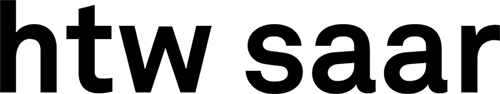
\includegraphics[width=3cm]{theme/htwlogo.png}
\end{frame}

\frameWithImageOnly{\BILDERPFAD/decorator1.jpg}

\begin{frame}{Beispielvorgehen bei der Erzeugung eines Getränks}
	\begin{block}{Wir möchten einen}
		\begin{itemize}
	 		\item Kaffee
	 		\item mit Milch
	 		\item mit Zucker
            \item mit Chili
	 	\end{itemize}
	\end{block}

	\pause
	\begin{exampleblock}{Was wir tun}
		\begin{enumerate}
	 		\item Nimm ein Kaffee-Objekt
	 		\item Dekoriere es mit Milch
	 		\item Dekoriere es mit Zucker
            \item Dekoriere es mit Chili
	 		\item Berechne Preis inklusive Milch, Zucker und Chili
	 	\end{enumerate}
 	\end{exampleblock}
\end{frame}

\begin{frame}{Allgemeines Klassendiagramm}
\begin{tikzpicture}[scale=0.8, transform shape]
    % Definiere eine Klasse
    \umlclass[x=6, y=0]{Komponente}{
    }{
        + methodeA() \\
        + methodeB() \\
    }

    % Definiere eine weitere Klasse
    \umlclass[x=0, y=-5]{KonkreteKomponente}{
    }{
        + methodeA() \\
        + methodeB() \\
    }

    \umlclass[x=5, y=-5]{Dekorierer}{
    }{
        + methodeA() \\
        + methodeB() \\
    }

    \umlclass[x=10, y=-2]{KonkreterDekorierer1}{
    }{
        + methodeA() \\
        + methodeB() \\
    }

    \umlclass[x=10, y=-5]{KonkreterDekorierer2}{
    }{
        + methodeA() \\
        + methodeB() \\
    }
    
    \umlinherit{KonkreteKomponente}{Komponente}
    \umlinherit{Dekorierer}{Komponente}
    \umlinherit{KonkreterDekorierer1}{Dekorierer}
    \umlinherit{KonkreterDekorierer2}{Dekorierer}
\end{tikzpicture}
\end{frame}

\begin{frame}{Klassendiagramm von Cafe King}
\begin{tikzpicture}[scale=0.6, transform shape]
    % Definiere eine Klasse
    \umlclass[x=6, y=0]{Beverage}{
    }{
        + getDescription(): String() \\
        + calculateCosts(): double \\
    }

    % Definiere eine weitere Klasse
    \umlclass[x=0, y=0]{Espresso}{
    }{
        + calculateCosts(): double\\
        + getDescription(): String() \\
    }

    \umlclass[x=0, y=-5]{Tea}{
    }{
        + calculateCosts(): double\\
        + getDescription(): String() \\
    }

    \umlclass[x=5, y=-5]{CondimentDecorator}{
    }{
    }

    \umlclass[x=14, y=-2]{MilkDecorator}{
    }{
        + getDescription(): String() \\
        + calculateCosts(): double \\
    }

    \umlclass[x=14, y=-5]{SugarDecorator}{
    }{
        + getDescription(): String() \\
        + calculateCosts(): double \\
    }
    
    \umlinherit{Espresso}{Beverage}
    \umlinherit{Tea}{Beverage}
    \umlinherit{CondimentDecorator}{Beverage}
    \umlinherit{SugarDecorator}{CondimentDecorator}
    \umlinherit{MilkDecorator}{CondimentDecorator}
\end{tikzpicture}
\end{frame}

\begin{frame}[fragile]{Grundlegende Schnittstelle}
	\begin{exampleblock}{Beverage.java}
        \begin{lstlisting}
public interface Beverage {
    String getDescription();
    double calculateCosts();
}
        \end{lstlisting}
	\end{exampleblock}
\end{frame}

\begin{frame}[fragile]{Konkrete Implementierung der Schnittstelle 1}
	\begin{exampleblock}{Coffee.java}
        \begin{lstlisting}
public class Coffee implements Beverage {
    @Override
    public String getDescription() {
        return "Normaler Kaffee";
    }

    @Override
    public double calculateCosts() {
        return 0.99;
    }
}
        \end{lstlisting}
	\end{exampleblock}
\end{frame}

\begin{frame}[fragile]{Konkrete Implementierung der Schnittstelle 2}
	\begin{exampleblock}{Espresso.java}
        \begin{lstlisting}
public class Espresso implements Beverage {
    @Override
    public String getDescription() {
        return "Espresso";
    }

    @Override
    public double calculateCosts() {
        return 1.99;
    }
}
        \end{lstlisting}
	\end{exampleblock}
\end{frame}

\begin{frame}[fragile]{Decorator-Abstraktion}
	\begin{exampleblock}{CondimentDecorator.java}
        \begin{lstlisting}
public abstract class CondimentDecorator implements Beverage {
    private Beverage beverage;

    public CondimentDecorator(Beverage beverage) {
        this.beverage = beverage;
    }

    public abstract String getDescription();
    
    protected Beverage getBeverage() {
		return beverage;
	}
}
        \end{lstlisting}
	\end{exampleblock}
\end{frame}

\begin{frame}[fragile]{Konkreter Dekorator 1}
	\begin{exampleblock}{MilkDecorator.java}
        \begin{lstlisting}
public class MilkDecorator extends CondimentDecorator {
    public MilkDecorator(Beverage beverage) {
        super(beverage);
    }

    @Override
    public String getDescription() {
        return getBeverage().getDescription() + ",  Milch";
    }

    @Override
    public double calculateCosts() {
        return getBeverage().calculateCosts() + 0.30;
    }
}
        \end{lstlisting}
	\end{exampleblock}
\end{frame}

\begin{frame}[fragile]{Konkreter Dekorator 2}
	\begin{exampleblock}{SugarDecorator.java}
        \begin{lstlisting}
public class SugarDecorator extends CondimentDecorator {
    public SugarDecorator(Beverage beverage) {
        super(beverage);
    }

    @Override
    public String getDescription() {
        return getBeverage().getDescription() + ", Zucker";
    }

    @Override
    public double calculateCosts() {
        return getBeverage().calculateCosts() + 0.10;
    }
}

        \end{lstlisting}
	\end{exampleblock}
\end{frame}

\begin{frame}[fragile]{Verwendung}
	\begin{exampleblock}{CoffeeDialog.java}
        \begin{lstlisting}
Beverage beverage = new Tea();
Beverage teaWithMilk = new MilkDecorator(beverage);
Beverage teaWithMilkAndCaramel = new CaramelDecorator(
    teaWithMilk);
Beverage teaWithMilkAndCaramelAndSoy = new SoyDecorator(
    teaWithMilkAndCaramel);
System.out.println("Das habe ich bestellt: " + 
    teaWithMilkAndCaramelAndSoy.getDescription());
System.out.println("Preis: " + 
    teaWithMilkAndCaramelAndSoy.calculateCosts());
        \end{lstlisting}
	\end{exampleblock}
\end{frame}

\frameWithImageOnly{\BILDERPFAD/decorator2.jpg}
\note{
    Als nächstes möchten wir ein kleines Nachrichtensystem implementieren. Nachrichten können verschlüsselt, komprimiert und als wichtig markiert werden. Markierung als wichtig bedeutet einfach nur ein Druck in Großbuchstaben.
}

\begin{frame}{Klassendiagramm}
\begin{tikzpicture}[scale=0.6, transform shape]
    % Definiere eine Klasse
    \umlclass[x=6, y=0]{Message}{
    }{
        + getContent(): String() \\
    }

    \umlclass[x=0, y=0]{SimpleMessage}{
    }{
        + getContent(): String() \\
    }

    \umlclass[x=0, y=-5]{MessageDecorator}{
    }{
        + getContent(): String() \\
    }

    \umlclass[x=5, y=-5]{EncryptionDecorator}{
    }{
        + getContent(): String() \\
    }

    \umlclass[x=14, y=-2]{CompressionDecorator}{
    }{
        + getContent(): String() \\
    }

    \umlclass[x=14, y=-5]{ImportantDecorator}{
    }{
        + getContent(): String() \\
    }
    
    \umlinherit{SimpleMessage}{Beverage}
    \umlinherit{Tea}{Message}
    \umlinherit{MessageDecorator}{Message}
    \umlinherit{EncryptionDecorator}{MessageDecorator}
    \umlinherit{CompressionDecorator}{MessageDecorator}
    \umlinherit{ImportantDecorator}{MessageDecorator}
\end{tikzpicture}
\end{frame}

\begin{frame}[fragile]{Grundlegende Schnittstelle}
	\begin{exampleblock}{Message.java}
        \begin{lstlisting}
public interface Message {
    String getContent();
}
        \end{lstlisting}
	\end{exampleblock}
\end{frame}

\begin{frame}[fragile]{Konkrete Implementierung der Schnittstelle}
	\begin{exampleblock}{SimpleMessage.java}
        \begin{lstlisting}
public class SimpleMessage implements Message {
    private String content;

    public SimpleMessage(String content) {
        this.content = content;
    }

    @Override
    public String getContent() {
        return content;
    }
}
        \end{lstlisting}
	\end{exampleblock}
\end{frame}

\begin{frame}[fragile]{Decorator-Abstraktion}
	\begin{exampleblock}{MessageDecorator.java}
        \begin{lstlisting}
public abstract class MessageDecorator implements Message {
    protected Message message;

    public MessageDecorator(Message message) {
        this.message = message;
    }

    @Override
    public String getContent() {
        return message.getContent();
    }
}

        \end{lstlisting}
	\end{exampleblock}
\end{frame}

\begin{frame}[fragile]{Konkreter Dekorator 1}
	\begin{exampleblock}{EncryptionDecorator.java}
        \begin{lstlisting}
public class EncryptionDecorator extends MessageDecorator {
    public EncryptionDecorator(Message message) {
        super(message);
    }

    @Override
    public String getContent() {
        return encrypt(message.getContent());
    }

    private String encrypt(String content) {
        return new StringBuilder(content).reverse().toString();
    }
}
        \end{lstlisting}
	\end{exampleblock}
\end{frame}

\begin{frame}[fragile]{Konkreter Dekorator 2}
	\begin{exampleblock}{ImportantDecorator.java}
        \begin{lstlisting}
public class ImportantDecorator extends MessageDecorator {
    public ImportantDecorator(Message message) {
        super(message);
    }

    @Override
    public String getContent() {
        return message.getContent().toUpperCase();
    }
}
        \end{lstlisting}
	\end{exampleblock}
\end{frame}

\frameWithImageOnly{\BILDERPFAD/decorator3.jpg}
\note{
    Systeme wie bspw. Nagios senden automatisch Benachrichtigungen an Administratoren, wenn z.B. ein Server ausfällt. Ein solches Nachrichtensystem soll im Folgenden im Kleinen mithilfe des Dekorators umgesetzt werden. 
}

\begin{frame}{Klassendiagramm}
\begin{tikzpicture}[scale=0.6, transform shape]
    % Definiere eine Klasse
    \umlclass[x=6, y=0]{Notifier}{
    }{
        + void send(String message); \\
    }

    \umlclass[x=0, y=0]{BasicNotifier}{
    }{
        + void send(String message); \\
    }

    \umlclass[x=0, y=-5]{NotifierDecorator}{
    }{
        + void send(String message); \\
    }

    \umlclass[x=14, y=0]{EmailNotifier}{
    }{
        + void send(String message); \\
    }

    \umlclass[x=14, y=-2]{SMSNotifier}{
    }{
        + void send(String message); \\
    }

    \umlclass[x=14, y=-5]{SlackNotifier}{
    }{
        + void send(String message); \\
    }
    
    \umlinherit{BasicNotifier}{Notifier}
    \umlinherit{NotifierDecorator}{Notifier}
    \umlinherit{EmailNotifier}{NotifierDecorator}
    \umlinherit{SMSNotifier}{NotifierDecorator}
    \umlinherit{SlackNotifier}{NotifierDecorator}
\end{tikzpicture}
\end{frame}

\begin{frame}[fragile]{Grundlegende Schnittstelle}
	\begin{exampleblock}{Notifier.java}
        \begin{lstlisting}
public interface Notifier {
    void send(String message);
}
        \end{lstlisting}
	\end{exampleblock}
\end{frame}

\begin{frame}[fragile]{Konkrete Implementierung der Schnittstelle}
	\begin{exampleblock}{BasicNotifier.java}
        \begin{lstlisting}
public class BasicNotifier implements Notifier {
    @Override
    public void send(String message) {
        System.out.println("...");
    }
}
        \end{lstlisting}
	\end{exampleblock}
\end{frame}

\begin{frame}[fragile]{Decorator-Abstraktion}
	\begin{exampleblock}{NotifierDecorator.java}
        \begin{lstlisting}
public class NotifierDecorator implements Notifier {
    private Notifier notifier;

    public NotifierDecorator(Notifier notifier) {
        this.notifier = notifier;
    }

    @Override
    public void send(String message) {
    	notifier.send(message);
    }
    
    public Notifier getNotifier() {
		return notifier;
	}
}
        \end{lstlisting}
	\end{exampleblock}
\end{frame}

\begin{frame}[fragile]{Konkreter Dekorator 1}
	\begin{exampleblock}{EmailNotifier.java}
        \begin{lstlisting}
public class EmailNotifier extends NotifierDecorator {
    public EmailNotifier(Notifier notifier) {
        super(notifier);
    }

    @Override
    public void send(String message) {
        super.send(message);
        sendEmail(message);
    }

    private void sendEmail(String message) {
        System.out.println("...");
    }
}
        \end{lstlisting}
	\end{exampleblock}
\end{frame}

\begin{frame}[fragile]{Konkreter Dekorator 2}
	\begin{exampleblock}{SMSNotifier.java}
        \begin{lstlisting}
public class SMSNotifier extends NotifierDecorator {
    public SMSNotifier(Notifier notifier) {
        super(notifier);
    }

    @Override
    public void send(String message) {
        super.send(message);
        sendSMS(message);
    }

    private void sendSMS(String message) {
        System.out.println("...");
    }
}
        \end{lstlisting}
	\end{exampleblock}
\end{frame}

\frameWithImageOnly{\BILDERPFAD/decorator4.jpg}
\note{
    Im folgenden Beispiel soll ein ähnlicher Effekt wie aspektorientierte Programmierung simuliert werden. Dort werden sog. Aspekte um bestehende Methoden gelegt werden, um beispielsweise Logging, Transaktionsmanagement oder Sicherheitsüberprüfungen hinzuzufügen.
}

\begin{frame}{Klassendiagramm Logging}
\begin{tikzpicture}[scale=0.6, transform shape]
    % Definiere eine Klasse
    \umlclass[x=6, y=0]{Service}{
    }{
        + void performOperation() \\
    }

    \umlclass[x=0, y=-3]{SimpleService}{
    }{
        + void performOperation() \\
    }

    \umlclass[x=6, y=-3]{ServiceDecorator}{
    }{
        + void performOperation() \\
    }

    \umlclass[x=6, y=-6]{LoggingDecorator}{
    }{
        + void performOperation() \\
    }

    \umlinherit{SimpleService}{Service}
    \umlinherit{ServiceDecorator}{Service}
    \umlinherit{LoggingDecorator}{ServiceDecorator}
\end{tikzpicture}
\end{frame}

\begin{frame}[fragile]{Grundlegende Schnittstelle}
	\begin{exampleblock}{Service.java}
        \begin{lstlisting}
public interface Service {
    void performOperation();
}
        \end{lstlisting}
	\end{exampleblock}
\end{frame}

\begin{frame}[fragile]{Konkrete Implementierung der Schnittstelle}
	\begin{exampleblock}{SimpleService.java}
        \begin{lstlisting}
public class SimpleService implements Service {
    @Override
    public void performOperation() {
        System.out.println("...");
        System.out.println("...");
    }
}
        \end{lstlisting}
	\end{exampleblock}
\end{frame}

\begin{frame}[fragile]{Decorator-Abstraktion}
	\begin{exampleblock}{ServiceDecorator.java}
        \begin{lstlisting}
public abstract class ServiceDecorator implements Service {
    private Service wrappee;

    public ServiceDecorator(Service service) {
        this.wrappee = service;
    }

    @Override
    public void performOperation() {
        wrappee.performOperation();
    }
}
        \end{lstlisting}
	\end{exampleblock}
\end{frame}

\begin{frame}[fragile]{Konkreter Dekorator}
	\begin{exampleblock}{LoggingDecorator.java}
        \begin{lstlisting}
public class LoggingDecorator extends ServiceDecorator {
    public LoggingDecorator(Service service) {
        super(service);
    }

    public void performOperation() {
        logBefore();
        super.performOperation();
        logAfter();
    }

    private void logBefore() {
        System.out.println("vorher");
    }

    private void logAfter() {
        System.out.println("nachher");
    }
}
        \end{lstlisting}
	\end{exampleblock}
\end{frame}
